\documentclass{article}
\usepackage[utf8]{inputenc}
\usepackage[german]{babel}
\usepackage{amsmath,amsthm,amssymb,mathrsfs}
\usepackage{geometry}
\usepackage[shortlabels]{enumitem}
\usepackage{wrapfig}

% For images
\usepackage{graphicx}
\usepackage{subcaption}
\graphicspath{ {./} }

% For tables not moving around
\usepackage{float}
\restylefloat{table}


\newcommand{\N}{\mathbb{N}}
\newcommand{\Q}{\mathbb{Q}}
\newcommand{\Z}{\mathbb{Z}}
\newcommand{\A}{\mathbb{A}}
\newcommand{\R}{\mathbb{R}}
\newcommand{\C}{\mathbb{C}}

\renewcommand{\i}{\text{i}}

\newcommand{\mat}[1]{\left(\begin{matrix}#1\end{matrix}\right)}
\newcommand{\smat}[1]{\left(\begin{smallmatrix}#1\end{smallmatrix}\right)}
\newcommand{\dmat}[1]{\begin{vmatrix}#1\end{vmatrix}}
\newcommand{\bmat}[2]{\left(\begin{array}{#1}#2\end{array}\right)}

\geometry{
	a4paper,
	total={170mm,240mm},
	left=20mm,
	top=30mm,
}


\begin{document}
	\begin{table}[h]
		\centering
		\begin{tabular*}{\textwidth}{@{\extracolsep{\fill}}l c r }
			Moritz Seppelt & & Computational Physics\\ 
			194557 & \textbf{\Large{Hausaufgabe 1}} & vom 01.11.2021\\
			\hline 
		\end{tabular*}
	\end{table}
	
	\begin{figure}[h]
		\centering
		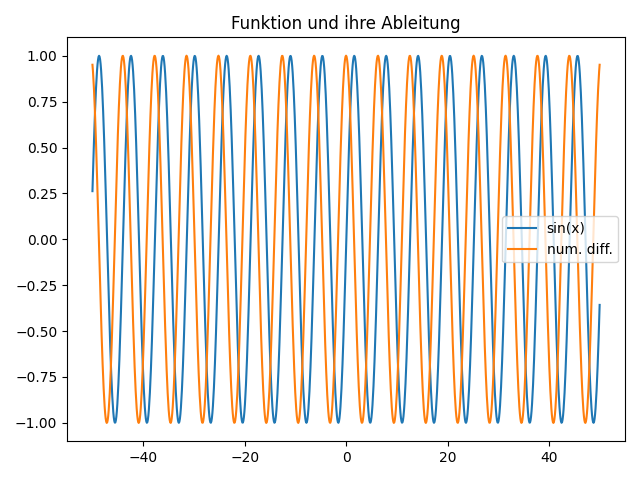
\includegraphics[scale=0.5]{Figure_1}
		\caption{Beispielergebnis numerische Differentation}
	\end{figure}
	In der Abbildung 1 wurde mit der blauen Linie $\sin(x)$ abgetragen und mit orange das Ergebnis der Berechnung der numerischen rechtsseitigen Differentiation. Diese Kurve ist genau $\frac{1}{4}$ Periode nach links verschoben. Sieht also genau so aus, wie $\cos(x)$. Nun wissen wir alle, dass
	$$\frac{\text{d}}{\text{d}x}\sin(x) = \cos(x)$$
	Somit erhalten wir in der Grafik das erwartete Ergebnis.
	
	Der Gesamtfehler $E$ ist definiert als
	$$ E_h = |f'(x) - D_h[f(x)]|\quad\text{mit } D_h[f(x)] = \frac{f(x+h)-f(x)}{h} $$
	\begin{wrapfigure}[12]{r}{0.4\textwidth}
		\centering
		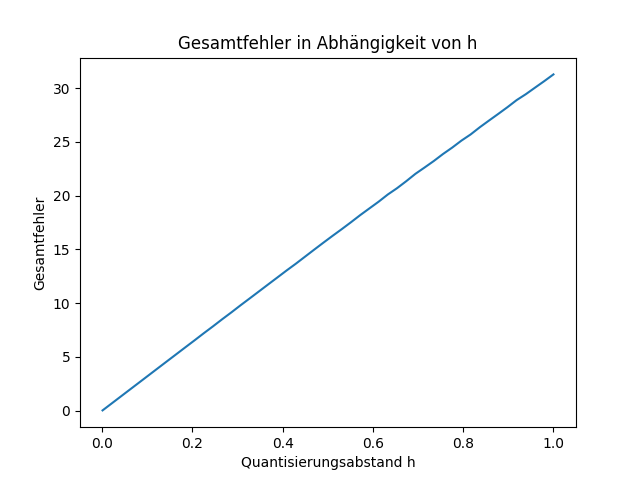
\includegraphics[width=0.4\textwidth]{Figure_2}
		\caption{Gesamtfehler in Abhängigkeit vum Quantisierungsabstand}
	\end{wrapfigure}
	Damit ergibt sich für den rechtsseitigen Differenzenquotienten folgender Zusammenhang mittels Taylor-Entwicklung:
	\begin{align*}
		f(x+h) &= f(x) + f'(x)h + \frac{1}{2}f''(x)h^2 + \frac{1}{6}f'''(x)h^3 + O(h^4)\\
		\Rightarrow D_h[f(x)] &= f'(x) + \frac{1}{2}f''(x)h+\frac{1}{6}f'''(x)h^2+O(h^3)\\
		\Rightarrow E_h &= \left| \frac{1}{2}f''(x)h+\frac{1}{6}f'''(x)h^2+O(h^3)\right|\\
		&\in O(h)
	\end{align*}

	Damit steigt der Fehler $E$ linear mit dem Quantisierungsabstand $h$, wie man in Abbildung 2 sieht. Am Ende sehen wie noch, dass der Fehler extrem ansteigt. Das liegt daran, dass der Abstand der Punkte, die für die Anstiegsberechnung hergenommen werden, so groß wird, dass eine Art Schwung entsteht, also dass die Ableitung extrem falsch wird. Was man auch in Abbildung 3a) sehen kann.
	
	Schließlich betrachten wir noch den lokalen Fehler der numerischen Differentation. Dafür sehen wir in Abbildung 3a jeweils den Fehler an einer Stelle für 3 verschiedene Quantisierungsabstände. In Abbildung 3b habe ich zum Vergleich die numerische und analytische Ableitung in einen Graphen geplottet (mit $h = 0,2$).
	
	\begin{figure}[H]
		\centering
		\subfloat[\centering Lokale Fehler]{{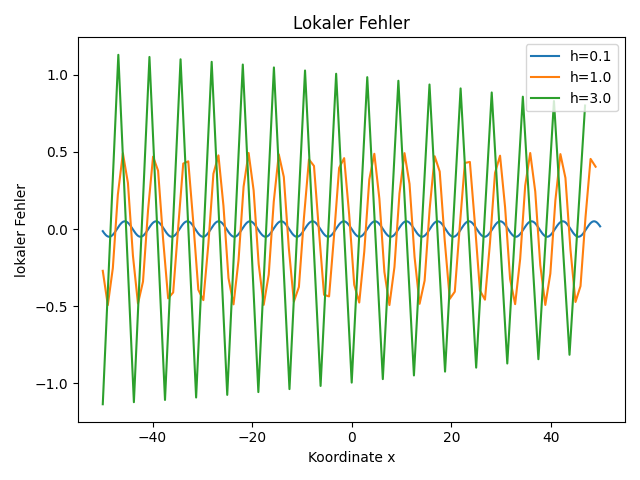
\includegraphics[scale=0.5]{Figure_3} }}
		\quad
		\subfloat[\centering analytische und numerische Ableitung für $h=0,2$]{{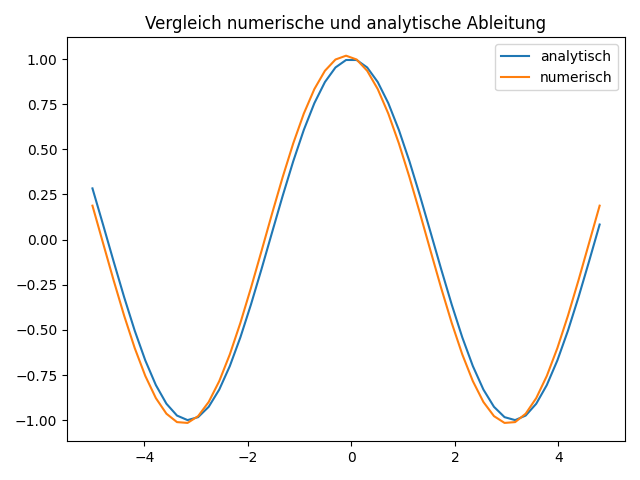
\includegraphics[scale=0.5]{Figure_4} }}
		\caption{Betrachtung der Lokalen Fehler}
	\end{figure}
	In 3a) sieht man, dass die lokale Fehler oszillieren und auch mit wachsendem $h$ linear steigen. Außerdem sieht man die Schwebung für $h=3$, die oben beschrieben wurde. Letzteres wissen wir ja schon aus der Abbildung 2. Bleibt noch die Frage, warum der lokale Fehler oszilliert. Dies kann Abbildung 3b) beantworten. Dort erkennt man, dass die numerische Approximation immer leicht nach links verschoben ist. Damit haben Stellen, wo die Ableitung einen kleinen Anstieg hat, natürlich nur einen kleinen lokalen Fehler. (vgl. mit $x=0$) Und an Stellen mit starker Steigung, ist auch der lokale Fehler größer. Da bei $\cos(x)$ diese Stellen oszillieren, tut dies auch der lokale Fehler
	
	\end{document}
